\documentclass[14pt]{extbook}
\usepackage{multicol, enumerate, enumitem, hyperref, color, soul, setspace, parskip, fancyhdr} %General Packages
\usepackage{amssymb, amsthm, amsmath, latexsym, units, mathtools} %Math Packages
\everymath{\displaystyle} %All math in Display Style
% Packages with additional options
\usepackage[headsep=0.5cm,headheight=12pt, left=1 in,right= 1 in,top= 1 in,bottom= 1 in]{geometry}
\usepackage[usenames,dvipsnames]{xcolor}
\usepackage{dashrule}  % Package to use the command below to create lines between items
\newcommand{\litem}[1]{\item#1\hspace*{-1cm}\rule{\textwidth}{0.4pt}}
\pagestyle{fancy}
\lhead{Progress Quiz 1}
\chead{}
\rhead{Version ALL}
\lfoot{3629-3146}
\cfoot{}
\rfoot{Summer C 2021}
\begin{document}

\begin{enumerate}
\litem{
Write the equation of the line in the graph below in Standard Form $Ax+By=C$. Then, choose the intervals that contain $A, B, \text{ and } C$.
\begin{center}
    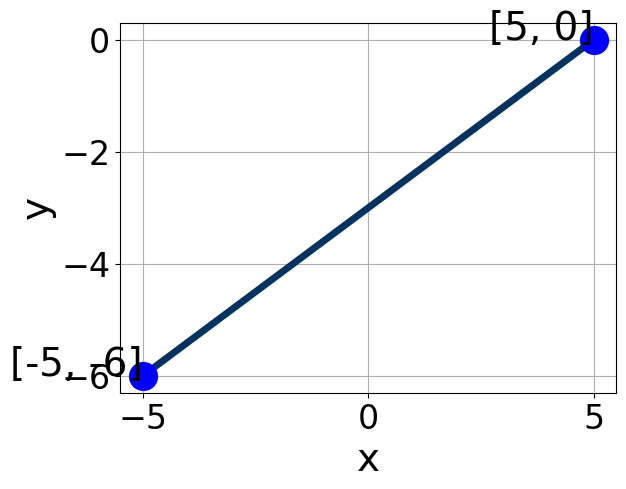
\includegraphics[width=0.5\textwidth]{../Figures/linearGraphToStandardA.png}
\end{center}
\begin{enumerate}[label=\Alph*.]
\item \( A \in [-0.1, 4.5], \hspace{3mm} B \in [4.6, 8], \text{ and } \hspace{3mm} C \in [-16, -12] \)
\item \( A \in [-1.8, -0.5], \hspace{3mm} B \in [-1.9, 0.2], \text{ and } \hspace{3mm} C \in [3, 8] \)
\item \( A \in [-1.8, -0.5], \hspace{3mm} B \in [0.3, 2.3], \text{ and } \hspace{3mm} C \in [-8, 2] \)
\item \( A \in [-5.1, -2.3], \hspace{3mm} B \in [4.6, 8], \text{ and } \hspace{3mm} C \in [-16, -12] \)
\item \( A \in [-0.1, 4.5], \hspace{3mm} B \in [-5.7, -4.3], \text{ and } \hspace{3mm} C \in [10, 21] \)

\end{enumerate} }
\litem{
Find the equation of the line described below. Write the linear equation in the form $ y=mx+b $ and choose the intervals that contain $m$ and $b$.\[ \text{Perpendicular to } 7 x - 8 y = 5 \text{ and passing through the point } (10, 9). \]\begin{enumerate}[label=\Alph*.]
\item \( m \in [-1.6, -0.99] \hspace*{3mm} b \in [19.4, 20.9] \)
\item \( m \in [-1.6, -0.99] \hspace*{3mm} b \in [-21.4, -18.8] \)
\item \( m \in [-1.6, -0.99] \hspace*{3mm} b \in [-1.3, 0.8] \)
\item \( m \in [-1, -0.6] \hspace*{3mm} b \in [19.4, 20.9] \)
\item \( m \in [0.64, 1.8] \hspace*{3mm} b \in [-3.4, -1.8] \)

\end{enumerate} }
\litem{
Solve the linear equation below. Then, choose the interval that contains the solution.\[ \frac{-6x -5}{7} - \frac{-7x + 5}{2} = \frac{4x -5}{4} \]\begin{enumerate}[label=\Alph*.]
\item \( x \in [-1.2, -0.5] \)
\item \( x \in [2.8, 3.7] \)
\item \( x \in [-3, -1.3] \)
\item \( x \in [0.1, 2.9] \)
\item \( \text{There are no real solutions.} \)

\end{enumerate} }
\litem{
Write the equation of the line in the graph below in Standard Form $Ax+By=C$. Then, choose the intervals that contain $A, B, \text{ and } C$.
\begin{center}
    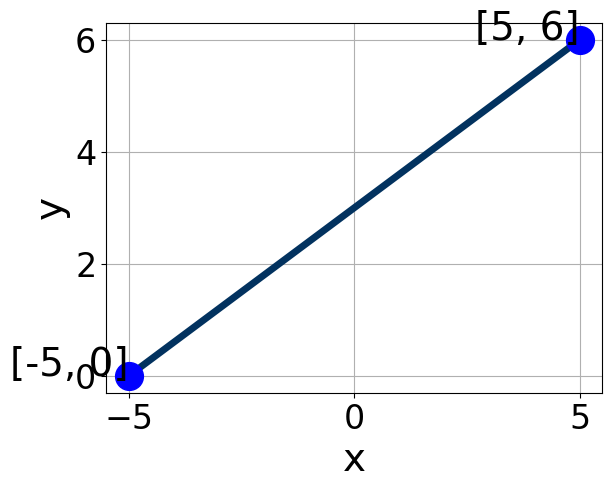
\includegraphics[width=0.5\textwidth]{../Figures/linearGraphToStandardCopyA.png}
\end{center}
\begin{enumerate}[label=\Alph*.]
\item \( A \in [-1.6, 2.4], \hspace{3mm} B \in [-2.4, -0.9], \text{ and } \hspace{3mm} C \in [-3, 2] \)
\item \( A \in [-1.6, 2.4], \hspace{3mm} B \in [0.2, 1.3], \text{ and } \hspace{3mm} C \in [-1, 4] \)
\item \( A \in [-4, -1], \hspace{3mm} B \in [4.1, 7.1], \text{ and } \hspace{3mm} C \in [15, 20] \)
\item \( A \in [2, 5], \hspace{3mm} B \in [4.1, 7.1], \text{ and } \hspace{3mm} C \in [15, 20] \)
\item \( A \in [2, 5], \hspace{3mm} B \in [-6.2, -4.8], \text{ and } \hspace{3mm} C \in [-17, -14] \)

\end{enumerate} }
\litem{
Find the equation of the line described below. Write the linear equation in the form $ y=mx+b $ and choose the intervals that contain $m$ and $b$.\[ \text{Parallel to } 5 x + 9 y = 15 \text{ and passing through the point } (-4, 8). \]\begin{enumerate}[label=\Alph*.]
\item \( m \in [-1.2, -0.25] \hspace*{3mm} b \in [11.1, 12.1] \)
\item \( m \in [-1.2, -0.25] \hspace*{3mm} b \in [4.7, 7.7] \)
\item \( m \in [-1.2, -0.25] \hspace*{3mm} b \in [-6.8, -4.5] \)
\item \( m \in [-2.76, -1.62] \hspace*{3mm} b \in [4.7, 7.7] \)
\item \( m \in [0.28, 1.49] \hspace*{3mm} b \in [10, 10.3] \)

\end{enumerate} }
\litem{
Solve the linear equation below. Then, choose the interval that contains the solution.\[ \frac{-7x -6}{6} - \frac{-7x -6}{5} = \frac{-3x -7}{7} \]\begin{enumerate}[label=\Alph*.]
\item \( x \in [-1.16, 0.31] \)
\item \( x \in [-11.22, -9.83] \)
\item \( x \in [0.78, 2.83] \)
\item \( x \in [-2.53, -1.78] \)
\item \( \text{There are no real solutions.} \)

\end{enumerate} }
\litem{
First, find the equation of the line containing the two points below. Then, write the equation in the form $ y=mx+b $ and choose the intervals that contain $m$ and $b$.\[ (-3, 6) \text{ and } (7, -11) \]\begin{enumerate}[label=\Alph*.]
\item \( m \in [-3.5, -0.8] \hspace*{3mm} b \in [-0.4, 4.1] \)
\item \( m \in [-3.5, -0.8] \hspace*{3mm} b \in [-19.6, -14.5] \)
\item \( m \in [1.6, 3] \hspace*{3mm} b \in [-25.8, -21.7] \)
\item \( m \in [-3.5, -0.8] \hspace*{3mm} b \in [-3.2, -0.1] \)
\item \( m \in [-3.5, -0.8] \hspace*{3mm} b \in [6.1, 10.3] \)

\end{enumerate} }
\litem{
Solve the equation below. Then, choose the interval that contains the solution.\[ -12(5x -2) = -9(15x + 7) \]\begin{enumerate}[label=\Alph*.]
\item \( x \in [-1.35, -1.05] \)
\item \( x \in [0.34, 0.63] \)
\item \( x \in [-0.53, -0.24] \)
\item \( x \in [-0.31, -0.12] \)
\item \( \text{There are no real solutions.} \)

\end{enumerate} }
\litem{
First, find the equation of the line containing the two points below. Then, write the equation in the form $ y=mx+b $ and choose the intervals that contain $m$ and $b$.\[ (-8, 5) \text{ and } (8, 4) \]\begin{enumerate}[label=\Alph*.]
\item \( m \in [-0.4, -0.02] \hspace*{3mm} b \in [12.97, 13.53] \)
\item \( m \in [0.04, 0.09] \hspace*{3mm} b \in [3.45, 4.08] \)
\item \( m \in [-0.4, -0.02] \hspace*{3mm} b \in [3.96, 4.57] \)
\item \( m \in [-0.4, -0.02] \hspace*{3mm} b \in [-4.05, -3.8] \)
\item \( m \in [-0.4, -0.02] \hspace*{3mm} b \in [-4.61, -4.44] \)

\end{enumerate} }
\litem{
Solve the equation below. Then, choose the interval that contains the solution.\[ -14(13x + 18) = -17(-4x -9) \]\begin{enumerate}[label=\Alph*.]
\item \( x \in [-0.79, 0.13] \)
\item \( x \in [-1.73, -1.55] \)
\item \( x \in [-1.15, -0.65] \)
\item \( x \in [0.34, 0.59] \)
\item \( \text{There are no real solutions.} \)

\end{enumerate} }
\litem{
Write the equation of the line in the graph below in Standard Form $Ax+By=C$. Then, choose the intervals that contain $A, B, \text{ and } C$.
\begin{center}
    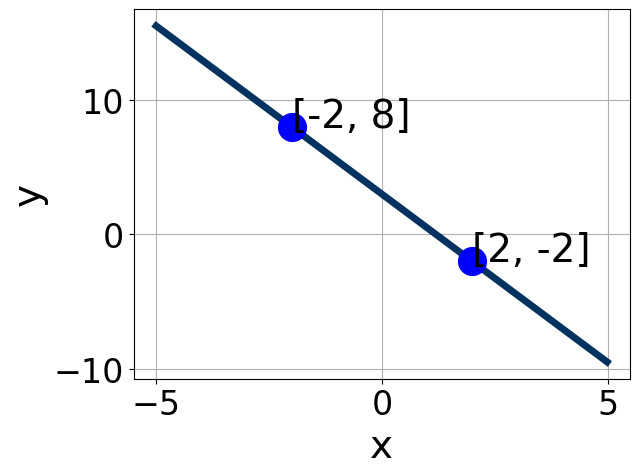
\includegraphics[width=0.5\textwidth]{../Figures/linearGraphToStandardB.png}
\end{center}
\begin{enumerate}[label=\Alph*.]
\item \( A \in [4, 7], \hspace{3mm} B \in [-3.08, -1.52], \text{ and } \hspace{3mm} C \in [-7.9, -5.6] \)
\item \( A \in [-8, 1], \hspace{3mm} B \in [-3.08, -1.52], \text{ and } \hspace{3mm} C \in [-7.9, -5.6] \)
\item \( A \in [-1.5, 4.5], \hspace{3mm} B \in [-0.21, 1.61], \text{ and } \hspace{3mm} C \in [1.6, 5.1] \)
\item \( A \in [4, 7], \hspace{3mm} B \in [1.83, 2.1], \text{ and } \hspace{3mm} C \in [5.1, 9.2] \)
\item \( A \in [-1.5, 4.5], \hspace{3mm} B \in [-1.55, -0.71], \text{ and } \hspace{3mm} C \in [-3.7, -1.5] \)

\end{enumerate} }
\litem{
Find the equation of the line described below. Write the linear equation in the form $ y=mx+b $ and choose the intervals that contain $m$ and $b$.\[ \text{Parallel to } 8 x - 7 y = 13 \text{ and passing through the point } (-7, 7). \]\begin{enumerate}[label=\Alph*.]
\item \( m \in [0.96, 1.48] \hspace*{3mm} b \in [13.02, 14.67] \)
\item \( m \in [-1.2, -0.85] \hspace*{3mm} b \in [-1.17, -0.99] \)
\item \( m \in [0.96, 1.48] \hspace*{3mm} b \in [-15.32, -14.66] \)
\item \( m \in [0.74, 1.11] \hspace*{3mm} b \in [14.79, 15.09] \)
\item \( m \in [0.96, 1.48] \hspace*{3mm} b \in [14.79, 15.09] \)

\end{enumerate} }
\litem{
Solve the linear equation below. Then, choose the interval that contains the solution.\[ \frac{-6x + 7}{2} - \frac{-5x + 7}{6} = \frac{-7x + 3}{8} \]\begin{enumerate}[label=\Alph*.]
\item \( x \in [-0.6, 0.5] \)
\item \( x \in [0.4, 3.3] \)
\item \( x \in [-4.2, -1.8] \)
\item \( x \in [1.6, 4] \)
\item \( \text{There are no real solutions.} \)

\end{enumerate} }
\litem{
Write the equation of the line in the graph below in Standard Form $Ax+By=C$. Then, choose the intervals that contain $A, B, \text{ and } C$.
\begin{center}
    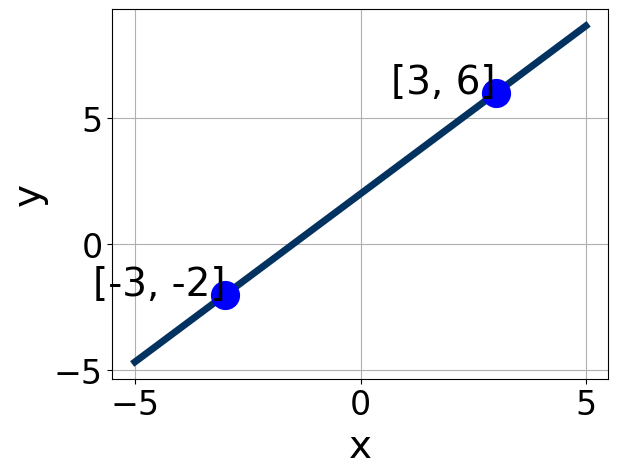
\includegraphics[width=0.5\textwidth]{../Figures/linearGraphToStandardCopyB.png}
\end{center}
\begin{enumerate}[label=\Alph*.]
\item \( A \in [-2.1, -1.2], \hspace{3mm} B \in [-2.7, -0.4], \text{ and } \hspace{3mm} C \in [-2.1, -0.5] \)
\item \( A \in [2.6, 7.1], \hspace{3mm} B \in [2.5, 5.2], \text{ and } \hspace{3mm} C \in [4.8, 9.5] \)
\item \( A \in [-2.1, -1.2], \hspace{3mm} B \in [0.5, 1.4], \text{ and } \hspace{3mm} C \in [-0.1, 2.9] \)
\item \( A \in [2.6, 7.1], \hspace{3mm} B \in [-3.2, -2.6], \text{ and } \hspace{3mm} C \in [-7.8, -4] \)
\item \( A \in [-4.9, -3.5], \hspace{3mm} B \in [2.5, 5.2], \text{ and } \hspace{3mm} C \in [4.8, 9.5] \)

\end{enumerate} }
\litem{
Find the equation of the line described below. Write the linear equation in the form $ y=mx+b $ and choose the intervals that contain $m$ and $b$.\[ \text{Parallel to } 7 x - 5 y = 7 \text{ and passing through the point } (7, -4). \]\begin{enumerate}[label=\Alph*.]
\item \( m \in [0.83, 2.03] \hspace*{3mm} b \in [12.9, 16.6] \)
\item \( m \in [-2.1, -1.18] \hspace*{3mm} b \in [5.4, 7.1] \)
\item \( m \in [0.59, 0.78] \hspace*{3mm} b \in [-15.3, -13.5] \)
\item \( m \in [0.83, 2.03] \hspace*{3mm} b \in [-15.3, -13.5] \)
\item \( m \in [0.83, 2.03] \hspace*{3mm} b \in [-11.2, -10.6] \)

\end{enumerate} }
\litem{
Solve the linear equation below. Then, choose the interval that contains the solution.\[ \frac{3x + 4}{3} - \frac{-7x -7}{5} = \frac{5x -9}{2} \]\begin{enumerate}[label=\Alph*.]
\item \( x \in [44.33, 46.33] \)
\item \( x \in [-4.45, -0.45] \)
\item \( x \in [67.33, 78.33] \)
\item \( x \in [197, 204] \)
\item \( \text{There are no real solutions.} \)

\end{enumerate} }
\litem{
First, find the equation of the line containing the two points below. Then, write the equation in the form $ y=mx+b $ and choose the intervals that contain $m$ and $b$.\[ (-2, -10) \text{ and } (-9, 11) \]\begin{enumerate}[label=\Alph*.]
\item \( m \in [2, 12] \hspace*{3mm} b \in [33, 41] \)
\item \( m \in [-6, -2] \hspace*{3mm} b \in [10, 17] \)
\item \( m \in [-6, -2] \hspace*{3mm} b \in [-20, -9] \)
\item \( m \in [-6, -2] \hspace*{3mm} b \in [-8, -6] \)
\item \( m \in [-6, -2] \hspace*{3mm} b \in [19, 23] \)

\end{enumerate} }
\litem{
Solve the equation below. Then, choose the interval that contains the solution.\[ -2(-8x + 12) = -5(-18x -16) \]\begin{enumerate}[label=\Alph*.]
\item \( x \in [-1.56, -1.34] \)
\item \( x \in [-1.1, -0.59] \)
\item \( x \in [0.61, 1.06] \)
\item \( x \in [-0.75, -0.25] \)
\item \( \text{There are no real solutions.} \)

\end{enumerate} }
\litem{
First, find the equation of the line containing the two points below. Then, write the equation in the form $ y=mx+b $ and choose the intervals that contain $m$ and $b$.\[ (7, -6) \text{ and } (10, -5) \]\begin{enumerate}[label=\Alph*.]
\item \( m \in [0.19, 0.59] \hspace*{3mm} b \in [-9.5, -7.3] \)
\item \( m \in [0.19, 0.59] \hspace*{3mm} b \in [-14.2, -12.1] \)
\item \( m \in [0.19, 0.59] \hspace*{3mm} b \in [6.3, 9.3] \)
\item \( m \in [0.19, 0.59] \hspace*{3mm} b \in [-16.5, -13.7] \)
\item \( m \in [-0.48, -0.14] \hspace*{3mm} b \in [-3, -0.1] \)

\end{enumerate} }
\litem{
Solve the equation below. Then, choose the interval that contains the solution.\[ -5(12x + 6) = -2(3x + 11) \]\begin{enumerate}[label=\Alph*.]
\item \( x \in [-0.22, 0] \)
\item \( x \in [-1.08, -0.8] \)
\item \( x \in [0.85, 1.13] \)
\item \( x \in [-0.81, -0.78] \)
\item \( \text{There are no real solutions.} \)

\end{enumerate} }
\litem{
Write the equation of the line in the graph below in Standard Form $Ax+By=C$. Then, choose the intervals that contain $A, B, \text{ and } C$.
\begin{center}
    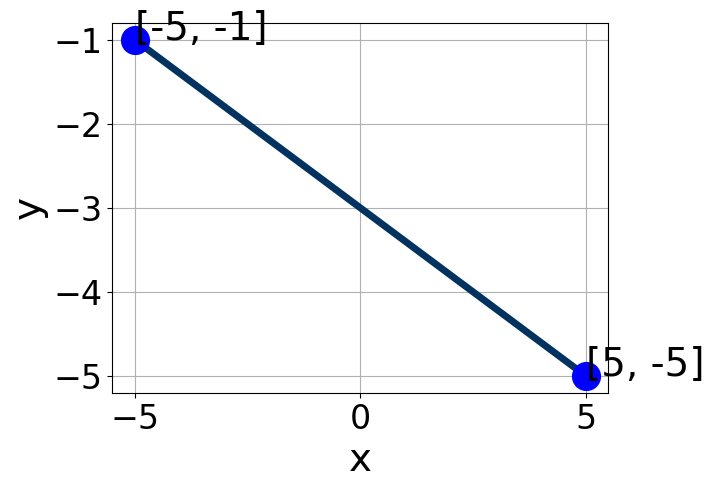
\includegraphics[width=0.5\textwidth]{../Figures/linearGraphToStandardC.png}
\end{center}
\begin{enumerate}[label=\Alph*.]
\item \( A \in [-0.5, 0.5], \hspace{3mm} B \in [-1.5, 0], \text{ and } \hspace{3mm} C \in [1, 5] \)
\item \( A \in [-4.2, -1.5], \hspace{3mm} B \in [-6.6, -3.8], \text{ and } \hspace{3mm} C \in [9, 19] \)
\item \( A \in [-0.5, 0.5], \hspace{3mm} B \in [0.2, 3.3], \text{ and } \hspace{3mm} C \in [-6, -2] \)
\item \( A \in [1.7, 2.2], \hspace{3mm} B \in [-6.6, -3.8], \text{ and } \hspace{3mm} C \in [9, 19] \)
\item \( A \in [1.7, 2.2], \hspace{3mm} B \in [3.5, 6.5], \text{ and } \hspace{3mm} C \in [-21, -13] \)

\end{enumerate} }
\litem{
Find the equation of the line described below. Write the linear equation in the form $ y=mx+b $ and choose the intervals that contain $m$ and $b$.\[ \text{Perpendicular to } 5 x - 7 y = 11 \text{ and passing through the point } (3, -9). \]\begin{enumerate}[label=\Alph*.]
\item \( m \in [-1.95, -0.92] \hspace*{3mm} b \in [-12.7, -11.3] \)
\item \( m \in [-1.95, -0.92] \hspace*{3mm} b \in [-5.4, -2.3] \)
\item \( m \in [1.19, 2.58] \hspace*{3mm} b \in [-14.4, -13.1] \)
\item \( m \in [-1.32, -0.04] \hspace*{3mm} b \in [-5.4, -2.3] \)
\item \( m \in [-1.95, -0.92] \hspace*{3mm} b \in [4.3, 7.1] \)

\end{enumerate} }
\litem{
Solve the linear equation below. Then, choose the interval that contains the solution.\[ \frac{-6x + 6}{7} - \frac{-3x + 4}{4} = \frac{4x -8}{5} \]\begin{enumerate}[label=\Alph*.]
\item \( x \in [-0.6, 1] \)
\item \( x \in [0.4, 1.9] \)
\item \( x \in [10.4, 12.3] \)
\item \( x \in [2.4, 4] \)
\item \( \text{There are no real solutions.} \)

\end{enumerate} }
\litem{
Write the equation of the line in the graph below in Standard Form $Ax+By=C$. Then, choose the intervals that contain $A, B, \text{ and } C$.
\begin{center}
    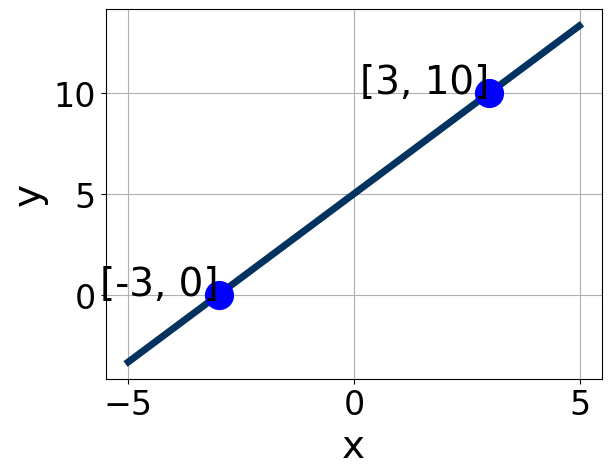
\includegraphics[width=0.5\textwidth]{../Figures/linearGraphToStandardCopyC.png}
\end{center}
\begin{enumerate}[label=\Alph*.]
\item \( A \in [-3, 0.3], \hspace{3mm} B \in [-0.5, 2.4], \text{ and } \hspace{3mm} C \in [0, 12] \)
\item \( A \in [-8.2, -1.7], \hspace{3mm} B \in [2.9, 3.9], \text{ and } \hspace{3mm} C \in [15, 26] \)
\item \( A \in [2.4, 5.7], \hspace{3mm} B \in [-3.7, -2.4], \text{ and } \hspace{3mm} C \in [-15, -13] \)
\item \( A \in [2.4, 5.7], \hspace{3mm} B \in [2.9, 3.9], \text{ and } \hspace{3mm} C \in [15, 26] \)
\item \( A \in [-3, 0.3], \hspace{3mm} B \in [-2.2, -0.9], \text{ and } \hspace{3mm} C \in [-8, -3] \)

\end{enumerate} }
\litem{
Find the equation of the line described below. Write the linear equation in the form $ y=mx+b $ and choose the intervals that contain $m$ and $b$.\[ \text{Parallel to } 9 x - 8 y = 7 \text{ and passing through the point } (-3, -5). \]\begin{enumerate}[label=\Alph*.]
\item \( m \in [1.01, 1.38] \hspace*{3mm} b \in [1.53, 1.73] \)
\item \( m \in [1.01, 1.38] \hspace*{3mm} b \in [-1.96, -1.53] \)
\item \( m \in [1.01, 1.38] \hspace*{3mm} b \in [-2.13, -1.8] \)
\item \( m \in [-0.45, 1.02] \hspace*{3mm} b \in [-1.96, -1.53] \)
\item \( m \in [-1.49, 0.54] \hspace*{3mm} b \in [-8.58, -8.29] \)

\end{enumerate} }
\litem{
Solve the linear equation below. Then, choose the interval that contains the solution.\[ \frac{-3x + 8}{3} - \frac{8x -9}{7} = \frac{-3x -9}{5} \]\begin{enumerate}[label=\Alph*.]
\item \( x \in [2.73, 5.73] \)
\item \( x \in [-1.28, 1.72] \)
\item \( x \in [1.06, 3.06] \)
\item \( x \in [15.85, 18.85] \)
\item \( \text{There are no real solutions.} \)

\end{enumerate} }
\litem{
First, find the equation of the line containing the two points below. Then, write the equation in the form $ y=mx+b $ and choose the intervals that contain $m$ and $b$.\[ (-4, -3) \text{ and } (8, -9) \]\begin{enumerate}[label=\Alph*.]
\item \( m \in [-0.54, 0.07] \hspace*{3mm} b \in [-8, -4] \)
\item \( m \in [0.44, 0.55] \hspace*{3mm} b \in [-13, -12] \)
\item \( m \in [-0.54, 0.07] \hspace*{3mm} b \in [-17, -15] \)
\item \( m \in [-0.54, 0.07] \hspace*{3mm} b \in [5, 7] \)
\item \( m \in [-0.54, 0.07] \hspace*{3mm} b \in [-3, 2] \)

\end{enumerate} }
\litem{
Solve the equation below. Then, choose the interval that contains the solution.\[ -15(-3x + 5) = -17(-19x + 11) \]\begin{enumerate}[label=\Alph*.]
\item \( x \in [0.79, 1.37] \)
\item \( x \in [0.05, 0.69] \)
\item \( x \in [-1.11, -0.94] \)
\item \( x \in [0.57, 0.93] \)
\item \( \text{There are no real solutions.} \)

\end{enumerate} }
\litem{
First, find the equation of the line containing the two points below. Then, write the equation in the form $ y=mx+b $ and choose the intervals that contain $m$ and $b$.\[ (-3, 9) \text{ and } (8, 2) \]\begin{enumerate}[label=\Alph*.]
\item \( m \in [-2.49, 0.19] \hspace*{3mm} b \in [10.07, 12.91] \)
\item \( m \in [0.47, 2.35] \hspace*{3mm} b \in [-3.67, -2.56] \)
\item \( m \in [-2.49, 0.19] \hspace*{3mm} b \in [-6.04, -5.31] \)
\item \( m \in [-2.49, 0.19] \hspace*{3mm} b \in [-7.21, -6.31] \)
\item \( m \in [-2.49, 0.19] \hspace*{3mm} b \in [6.55, 7.96] \)

\end{enumerate} }
\litem{
Solve the equation below. Then, choose the interval that contains the solution.\[ -15(13x + 14) = -12(-5x -16) \]\begin{enumerate}[label=\Alph*.]
\item \( x \in [-0.25, -0.11] \)
\item \( x \in [-0.12, -0.05] \)
\item \( x \in [-1.67, -1.46] \)
\item \( x \in [0.01, 0.09] \)
\item \( \text{There are no real solutions.} \)

\end{enumerate} }
\end{enumerate}

\end{document}